\documentclass[12pt]{article}

\usepackage{hyperref}
\usepackage[width=6in,height=9in]{geometry}
\usepackage{graphicx}
\usepackage{float}

\usepackage{tabularx}
\usepackage{booktabs}

\usepackage{tikz}
\usepackage{amsmath}
\usepackage{amsthm}
\theoremstyle{definition}
\newtheorem{exercise}{Exercise}
\newtheorem*{example}{Example}


\title{Keys and The Circle of Fifths}
\author{Addison Ballif}
\date{\today}

\begin{document}

\maketitle

There is a lot of structure in music. As this structure is commonly reused in different pieces, it is very useful to be aware of many of the patterns that go on. In this document I hope to explain the concept of 
\begin{itemize}
\item keys,
\item how notes fit into each key,
\item chords and their purpose,
\item how to know which chords to use.
\end{itemize}
This document should hopefully help open your ears to hear music in a new way. 

\section{Background}
Before we can talk about keys we need to first talk about notes and the difference between notes and chords. 

\vspace{0.5cm}
\noindent
\begin{tabularx}{\textwidth}{ 
  >{\hsize=0.75\hsize}X 
  >{\hsize=1.25\hsize}X 
}
    \toprule
    \textbf{Notes} & \textbf{Chords} \\
    \midrule
    A note is a pitch with a specific frequency. & A chord is a collection of frequencies at the same time. \\ \addlinespace
    We can sing notes. & We cannot sing chords, though instruments such as piano and guitar can play chords. \\ \addlinespace
    Each note has a name. & The name of the chord depends on the notes in the chord, and one chord may have multiple names. \\
    \bottomrule
\end{tabularx}
\vspace{0.5cm}

\newpage
Below is a piano keyboard that gives the ordering of the different notes and their names. 

\begin{center}

\includegraphics[width=0.9\linewidth]{keyboard.png}
\end{center}

As you can see on the keyboard above, we label the notes using 7 letters of the alphabet. (You can ignore the numbers on the figure for now.)
On the piano we label the white keys with the letters A through G, and then repeat. There are a five notes that lie in between the white keys. These are labeled by taking the note below (or above) and adding a sharp $\sharp$ (or a flat $\flat$) to the note. 
Because these notes can be labeled above or below, they have two names to represent the same thing. 
$$ \text C \sharp = \text D \flat, \hspace{0.5cm} \text D \sharp = \text E \flat, \hspace{0.5cm} \text F \sharp = \text G \flat, \hspace{0.5cm} \text{etc.}$$
This may seem redundant, but it is important to have both when we get to creating scales of notes. 

Notice that after 12 notes the pattern repeats. The piano keyboard looks exactly the same after playing each of the 12 notes (including the black keys). The distance of 12 notes is called an octave. 

\newpage
\section{Keys and Tonal Centers}

Much of the music we listen to today has what is called a key. 
The key is the tonal center for the music. 
The key is a single note that represents the home or root pitch for the tune. 
Everything in a piece of music is relative to the key. Recognizing this allows us to look for patterns between pieces of music 
that may be in different keys. 
In this document we will explore common structure found in popular music. 

\begin{example}
Below are a few popular songs and their keys. 
Listen to each of these songs. Then using a drone\footnote{You can find a tool for creating drone notes \href{https://ahballif.github.io/AddisonGuitarResources/drones.html}{on my website.}}
, or an instrument such as a piano or guitar, listen to the key note and pay attention to 
how the song is centered around that note. 
\begin{itemize}
\item \href{https://www.youtube.com/watch?v=tiBaBca7-rY}{``Son of Man'' by Phil Collins.} The starting key is in D. At 1:36 the key changes to E.
\item \href{https://www.youtube.com/watch?v=ElN_4vUvTPs}{``Human Nature'' by Michael Jackson.} This song is in the key of D.

\item \href{https://www.youtube.com/watch?v=sKljOD5B71k}{``Nemo Egg'' by Thomas Newman.} This song is in the key of F.

\item \href{https://www.youtube.com/watch?v=KuAAroUML0g}{``Moonlight in Vermont'' performed by Frank Sinatra.} He sings this song in D$\flat$. 

\item \href{https://www.youtube.com/watch?v=WJCw-lvuS-c}{``Moonlight in Vermont'' performed by Ella Fitzgerald. } She sings it in C.

\end{itemize}
\end{example}

Notice in the example above the last two selections, which are the same piece but in (slightly) different keys. 
It is common for singers to change the key of a song in order to fit their vocal range. 
Doing so does not change the recognizability or structure of the melody. 


\begin{exercise} \label{ex:findkeys}
With the aid of a keyboard or notemaking tool, identify the key of the following tunes. 
\begin{itemize}
\item \href{https://www.youtube.com/watch?v=xUNqsfFUwhY}{``Here Comes The Sun'' by the Beatles.}
\item \href{https://www.youtube.com/watch?v=hNvN8uAIUQ4}{``We Are Family'' by Sister Sledge.}
\item \href{https://www.youtube.com/watch?v=muOpokalL0s}{``Let's Fall In Love'' performed by Diana Krall.}
\item \href{https://www.youtube.com/watch?v=CbGy_Vf1HgU}{``The Precious Jewel'' by Pat Metheny and Charlie Haden.}
\end{itemize}
\end{exercise}

You can find the answers for this exercise at the end of this document.

\newpage
\section{The Major Scale}
Once the key has been identified, we then need a way of describing the overall sound of the song in that key.
This is determined by the other notes that we choose to include. 
The two most common sounds we can create in a key are major and minor. 
The major scale is typically described as having a ``happier'' sound while the minor has a more ``sad'' sound. 
It is true that major is a brighter sound than the minor. 

We often describe the other notes in the key by identifying a scale. 
The scale refers to all the notes allowed for a given key, and is usually played in an ascending or descending pattern.

\begin{example}
The C major scale consists of the notes C, D, E, F, G, A, B. These notes are then repeated in the next octave. 
The white notes of the piano are designed to play the C major scale. 
\end{example}

In the preceding example we give the notes of the major scale for C major. 
Let us look more closely as the distances between the notes. 
On the piano keyboard the distance between two notes is called a half step (for example the distance between C and C$\sharp$, or E and F).
Analysing the distances between the notes of the C major scale, we find the following sequence of half-step jumps:
\[
\text{C} 
\underbrace{\quad}_{2} \text{D} 
\underbrace{\quad}_{2} \text{E} 
\underbrace{\quad}_{1} \text{F} 
\underbrace{\quad}_{2} \text{G} 
\underbrace{\quad}_{2} \text{A} 
\underbrace{\quad}_{2} \text{B} 
\underbrace{\quad}_{1} \text{C}
\]
with the last note taking us back to the root note in the higher octave. We can use this same spacing of half steps to create a major scale in any key.

\begin{example}
The D major scale consists of the notes 
\[
\text{D} 
\underbrace{\quad}_{2} \text{E} 
\underbrace{\quad}_{2} \text{F$\sharp$} 
\underbrace{\quad}_{1} \text{G} 
\underbrace{\quad}_{2} \text{A} 
\underbrace{\quad}_{2} \text{B} 
\underbrace{\quad}_{2} \text{C$\sharp$} 
\underbrace{\quad}_{1} \text{D}
\]
\end{example}

\begin{exercise} \label{ex:writeScales}
Using the sequences of half step jumps and the piano keyboard given above, write down the note names for a major scale starting on each of the 12 notes. For the notes that have multiple names, choose the names so that each letter is only used once, and moving from one note to the next moves to the next letter of the alphabet. For example, if the root is B, we would choose C$\sharp$ as the second note rather than D$\flat$. 
\end{exercise}

From now on we will want to refer to notes based on how they would fit in the major scale. 
For example we might say ``play the third of the key,'' which would mean to play the third note of the major scale for that key. 
As we go on, we will want to shift from thinking about notes using their letter names but instead based on how they fall in comparison to the major scale of the key. 
To help you get used to this idea, the following exercises are designed to help you move between note names and scale degrees in this way.

\begin{exercise}
Using my \href{https://ahballif.github.io/AddisonGuitarResources/scale_degree_keys.html}{online scale degree quiz,} practice identifying the scale degree based on the note name using the quiz on the right of the page. You may use the piano keyboard chart to help you. Try include more keys by selecting them in the settings box at the bottom of the page. Do not include chromatic notes. 
\end{exercise}

\begin{exercise}
Similar to the previous exercise, use the \href{https://ahballif.github.io/AddisonGuitarResources/scale_degree_keys.html}{online scale degree quiz} to practice identifying the note name based on the scale degree using the quiz on the left of the page. 
\end{exercise}

As we transition from thinking of specific notes with their letter names to thinking of notes in terms of their relationship to the root of the key, we can start training a skill known as relative pitch. This is the ability to hear notes based on their relationship to the root, even without knowing what their absolute pitch or letter name is. The next exercise is designed to help you start training this skill. 

\begin{exercise}
Use the \href{https://ahballif.github.io/AddisonGuitarResources/scale_degree_ear_quiz.html}{online ear training quiz} to practice identifying scale degrees by ear.
\end{exercise}

\subsection{Key Signatures}
In Exercise \ref{ex:writeScales} you named the notes of each of the major scales. You should have noticed that by using the rule that each letter is only used once, a scale only has flats or sharps but not both. The number of flats or sharps is called the key signature. 
We might say ``the key signature has 3 flats'' and if that were so then we would call the key E$\flat$ major. 

\begin{exercise}
Sharps and flats are added to a key signature. Determine the order that sharps are added and the order that flats are added. 
For example, the first sharp to be added is F$\sharp$ since G major has one sharp. D major is the key with two sharps, and the first one is F$\sharp$. What is the second?
\end{exercise}

\newpage
\section{The Circle of Fifths}
A powerful way of organizing the twelve different keys is using a cycle structure known as the circle of fifths (or circle of fourths). 
The circle is shown below. 

\begin{center}
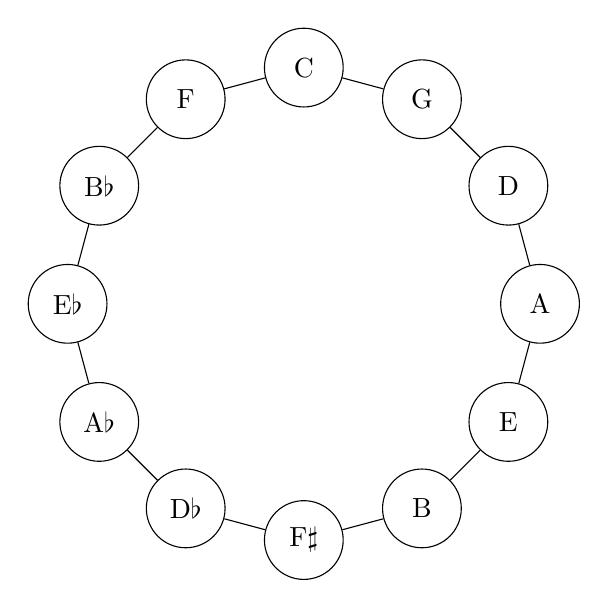
\begin{tikzpicture}[every node/.style={draw, circle, minimum size=1cm}, scale = 1.5]

\node (v0) at (0*-30+90:2cm) {C};
\node (v1) at (1*-30+90:2cm) {G};
\node (v2) at (2*-30+90:2cm) {D};
\node (v3) at (3*-30+90:2cm) {A};
\node (v4) at (4*-30+90:2cm) {E};
\node (v5) at (5*-30+90:2cm) {B};
\node (v6) at (6*-30+90:2cm) {F$\sharp$};
\node (v7) at (7*-30+90:2cm) {D$\flat$};
\node (v8) at (8*-30+90:2cm) {A$\flat$};
\node (v9) at (9*-30+90:2cm) {E$\flat$};
\node (v10) at (10*-30+90:2cm) {B$\flat$};
\node (v11) at (11*-30+90:2cm) {F};

\foreach \i in {0,...,10} {
    \draw (v\i) -- (v\the\numexpr\i+1\relax);
}
\draw (v11) -- (v0);

\end{tikzpicture}
\end{center}

The ordering of the notes is chosen so that each of the notes is a fourth or fifth away (depending on whether you move up or down).
This choice creates some useful structure, and there are several things we can notice. 
There are several things we can notice about the structure. 
\begin{itemize}
\item Every time we move clockwise we lose one flat or gain one sharp.
\item Every time we move counterclockwise we lose one sharp or gain one flat.
\item The clockwise follows the order that sharps are added starting on F. 
\item the order counter clockwise follows the order that flats are added starting on B. 
\end{itemize}

\begin{exercise}
Repeat Exercise \ref{ex:writeScales} but do it in the order given by the circle of fifths, and use the circle and the things you have learned about key signatures to help you. You should find that this process is quicker than counting the number of half steps between notes. 
\end{exercise}

\subsection*{Popular Chords}
The circle of fifths also identifies many patterns that we find in popular music. One common question would be how the chords in a popular song relate to each other. Many popular music uses what is commonly refered to as the "four chords," but how do we find these four chords for any given key? Consider the circle drawn below and suppose we are playing in the key of G major. The four chords we would use are highlighed.

\begin{center}
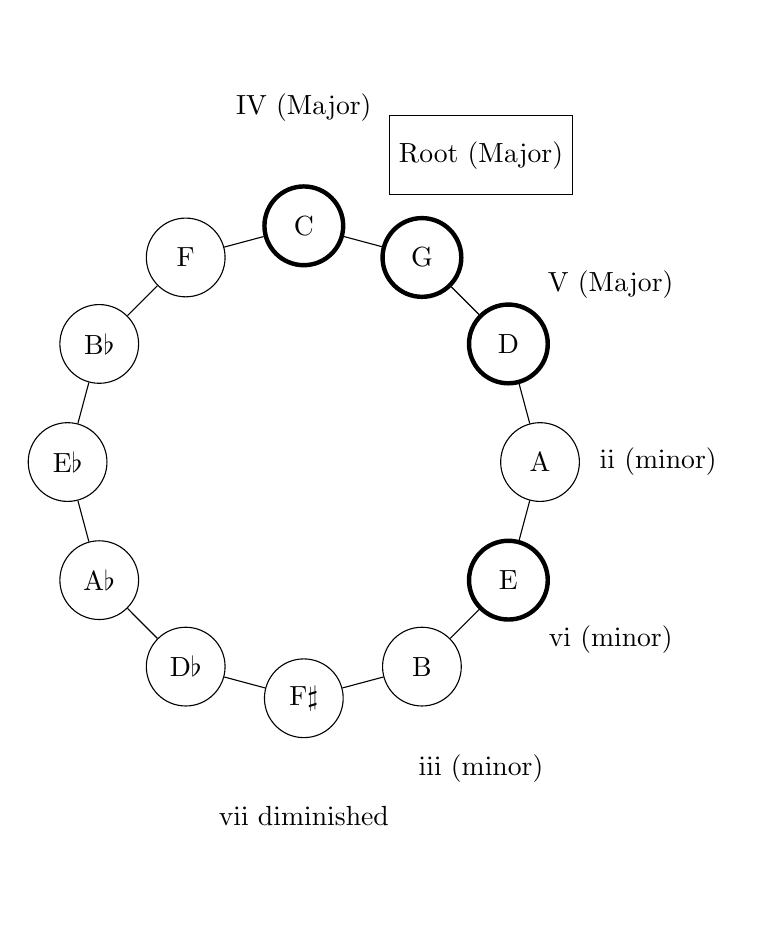
\begin{tikzpicture}[every node/.style={draw, circle, minimum size=1cm}, scale = 1.5]

\node[ultra thick] (v0) at (0*-30+90:2cm) {C}; \node[draw=none](w0) at (0*-30+90:3cm) {IV (Major)};
\node[ultra thick] (v1) at (1*-30+90:2cm) {G}; \node[rectangle](w1) at (1*-30+90:3cm) {Root (Major)};
\node[ultra thick] (v2) at (2*-30+90:2cm) {D}; \node[draw=none](w2) at (2*-30+90:3cm) {V (Major)};
\node (v3) at (3*-30+90:2cm) {A}; \node[draw=none](w3) at (3*-30+90:3cm) {ii (minor)};
\node[ultra thick] (v4) at (4*-30+90:2cm) {E}; \node[draw=none](w4) at (4*-30+90:3cm) {vi (minor)};
\node (v5) at (5*-30+90:2cm) {B}; \node[draw=none](w5) at (5*-30+90:3cm) {iii (minor)};
\node (v6) at (6*-30+90:2cm) {F$\sharp$}; \node[draw=none](w5) at (6*-30+90:3cm) {vii diminished};
\node (v7) at (7*-30+90:2cm) {D$\flat$};
\node (v8) at (8*-30+90:2cm) {A$\flat$};
\node (v9) at (9*-30+90:2cm) {E$\flat$};
\node (v10) at (10*-30+90:2cm) {B$\flat$};
\node (v11) at (11*-30+90:2cm) {F};

\foreach \i in {0,...,10} {
    \draw (v\i) -- (v\the\numexpr\i+1\relax);
}
\draw (v11) -- (v0);

\end{tikzpicture}
\end{center}

Notice the structure. 
\begin{center}
    The four chords are determined by the root and its two neighbors, as well as the minor chord 4 notes in the clockwise direction.
\end{center} 
Thus in G major we would have G, C, D, and E minor as our four chords. 
If we keep the structure the same but rotate only the notes, we can find the 4 chords for any possible key. 

We might also label these chords based on their scale degree. In G major, C would make the IV chord, D would make the V chord, and Em would make the vi chord. We often use capital Roman numerals for major chords and lower case Roman numerals for minor chords. 

Whenever we are playing in a major key, the chords for the two notes on either side of the root will also be major chords. The three to the right of the major chords are then the minor chords we could use in that key. Occationally (though not as common in pop music) we may need the seventh chord which is diminished. Some songs will use the ii chord or iii chord, so it is good to know that those are minor. 
This set of seven possible chords one could play in a key is known as the diatonic chords because they only play notes that are inside the scale for the key. 

\begin{exercise} \label{ex:fourChords}
Find the four pop chords for all of the 12 major keys using the circle of fifths. 
\end{exercise}



\newpage
\section{Exercise Answers}
Exercise \ref{ex:findkeys}: 
\begin{itemize}
\item``Here Comes The Sun'' is in A. 
\item``We Are Family'' is in A. 
\item``Let's Fall In Love'' is in E$\flat$. 
\item``The Precious Jewel'' is in E for the melody, and changes to C for the guitar solo. 
\end{itemize}

Exercise \ref{ex:writeScales}: Below are all of the major scales.
\begin{itemize}
\item C, D, E, F, G, A, B, C
\item D$\flat$, E$\flat$, F, G$\flat$, A$\flat$, B$\flat$, C, D$\flat$
\item D, E, F$\sharp$, G, A, B, C$\sharp$, D
\item E$\flat$, F, G, A$\flat$, B$\flat$, C, D, E$\flat$
\item E, F$\sharp$, G$\sharp$, A, B, C$\sharp$, D$\sharp$, E
\item F, G, A, B$\flat$, C, D, E, F
\item F$\sharp$, G$\sharp$, A$\sharp$, B, C$\sharp$, D$\sharp$, E$\sharp$, F$\sharp$
\item OR G$\flat$, A$\flat$, B$\flat$, C$\flat$, D$\flat$, E$\flat$, F, G$\flat$
\item G, A, B, C, D, E, F$\sharp$, G
\item A$\flat$, B$\flat$, C, D$\flat$, E$\flat$, F, G, A$\flat$
\item A, B, C$\sharp$, D, E, F$\sharp$, G$\sharp$, A
\item B$\flat$, C, D, E$\flat$, F, G, A, B$\flat$
\item B, C$\sharp$, D$\sharp$, E, F$\sharp$, G$\sharp$, A$\sharp$, B
\end{itemize}
When doing this exercise, we usually choose note names that are one letter above the previous note so that no letters are repeated. That is why in D$\flat$ major we would choose F and then G$\flat$ rather than F and the F$\sharp$. 

Exercise \ref{ex:fourChords}: Here are the four chords in each key. 
\begin{itemize}
    \item \textbf{C Major:} C, G, Am, F
    \item \textbf{G Major:} G, D, Em, C
    \item \textbf{D Major:} D, A, Bm, G
    \item \textbf{A Major:} A, E, F$\sharp$m, D
    \item \textbf{E Major:} E, B, C$\sharp$m, A
    \item \textbf{B Major:} B, F$\sharp$, G$\sharp$m, E
    \item \textbf{F$\sharp$ Major:} F$\sharp$, C$\sharp$, D$\sharp$m, B
    \item \textbf{D$\flat$ Major:} D$\flat$, A$\flat$, B$\flat$m, G$\flat$
    \item \textbf{A$\flat$ Major:} A$\flat$, E$\flat$, Fm, D$\flat$
    \item \textbf{E$\flat$ Major:} E$\flat$, B$\flat$, Cm, A$\flat$
    \item \textbf{B$\flat$ Major:} B$\flat$, F, Gm, E$\flat$
    \item \textbf{F Major:} F, C, Dm, B$\flat$
\end{itemize}

\end{document}
